\documentclass[a4paper,10pt]{article}
\usepackage[utf8]{inputenc}
\usepackage[T1]{fontenc}	
\usepackage[italian]{babel}

\usepackage{amsmath}
\usepackage{amsfonts}
\usepackage{amssymb}
\usepackage{graphicx}

\usepackage[left=2cm,right=2cm,top=2cm,bottom=2cm]{geometry}
\geometry{a4paper}

\usepackage{booktabs}
\usepackage{verbatim}
\usepackage{subfig}
\usepackage[italian, sort, noabbrev, capitalise]{cleveref}

\usepackage[cdot, thickqspace, squaren]{SIunits}
\usepackage{float}

% macro
\def\code#1{\texttt{#1}}

\title{Esercitazione 11: Semplici circuiti logici e Multivibratori.}
\author{Gruppo BL \\ Candido Alessandro, Luzio Andrea, Mazziotti Fabrizio}

\begin{document}

\maketitle

\section{Scopo e Strumentazione}
Studio dell'applicazione delle porte NAND nella costruzione di semplici circuiti logici e multivibratori.

La strumentazione è quella solitamente presente sul banco di lavoro, e inoltre si è usato:
\begin{itemize}
	\item 2 circuiti integrati \code{SN7400} Quad-NAND Gate;
	\item 1 DIP Switch a 4 interuttori;
	\item 1 diodo \code{1N4148};
	\item 2 diodi LED;
	\item Impulsatore, realizzato nella precedente esperienza;
\end{itemize}

\section{Costruzione di circuiti logici elementari}
Si sono connessi due interruttori tra i due ingressi di una porta NAND, alimentata a $\unit{4.94 \pm 0.03}{\volt}$, e massa e si è posto un diodo LED, con una resistenza di protezione di $\sim \unit{330}{\ohm}$, all'uscita della porta.
Si è verificata la tabella di verità del NAND provando tutte le combinazioni delle posizioni dei due interruttori, verificando lo stato dell'uscita mediante l'accensione del LED.

Si è applicato lo stesso metodo anche gli altri circuiti descritti in questa sezione, e si è verificata la tabella di verità nei vari casi.
Inoltre si è usato l'impulsatore per visualizzare il risultato sull'oscilloscopio; si riportano i grafici nelle \cref{fig:AND,fig:OR,fig:XOR,fig:ADDER}.

\paragraph{AND} Si è realizzato il circuito AND con 2 porte NAND.

\begin{figure}[H]
	\centering
	\begin{minipage}{0.49\textwidth}
		\centering
		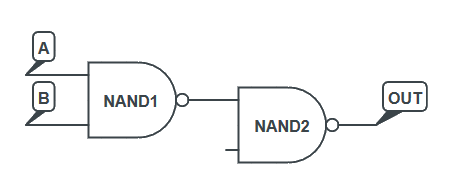
\includegraphics[width=\textwidth]{../grafici/AND1.png}
	\end{minipage}
	\begin{minipage}{0.49\textwidth}
		\centering
		\includegraphics[width=\textwidth]{../grafici/ANDard.pdf}
	\end{minipage}
	\caption{Schema del circuito AND e visualizzazione segnali in I/O}
	\label{fig:AND}
\end{figure}

\paragraph{OR} Si è realizzato il circuito OR con 3 porte NAND.

\begin{figure}[H]
	\centering
	\begin{minipage}{0.49\textwidth}
		\centering
		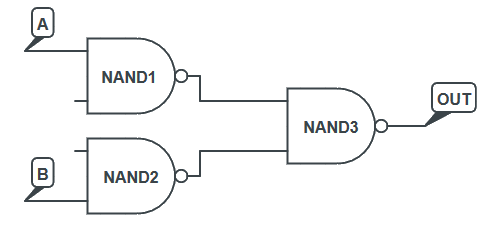
\includegraphics[width=\textwidth]{../grafici/OR1.png}
	\end{minipage}
	\begin{minipage}{0.49\textwidth}
		\centering
		\includegraphics[width=\textwidth]{../grafici/ORard.pdf}
	\end{minipage}
	\caption{Schema del circuito OR e visualizzazione segnali in I/O}
	\label{fig:OR}
\end{figure}

\paragraph{XOR} Si è realizzato il circuito XOR con 4 porte NAND.

\begin{figure}[H]
	\centering
	\begin{minipage}{0.49\textwidth}
		\centering
		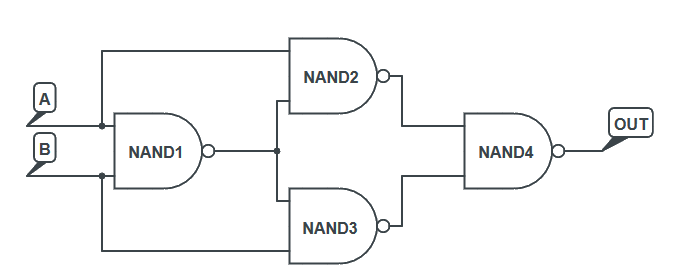
\includegraphics[width=\textwidth]{../grafici/XOR1.png}
	\end{minipage}
	\begin{minipage}{0.49\textwidth}
		\centering
		\includegraphics[width=\textwidth]{../grafici/XORard.pdf}
	\end{minipage}
	\caption{Schema del circuito XOR e visualizzazione segnali in I/O}
	\label{fig:XOR}
\end{figure}


\paragraph{Sommatore ad un bit} Si è realizzato il sommatore ad un bit con 5 porte NAND.

\begin{figure}[H]
	\centering
	\begin{minipage}{0.49\textwidth}
		\centering
		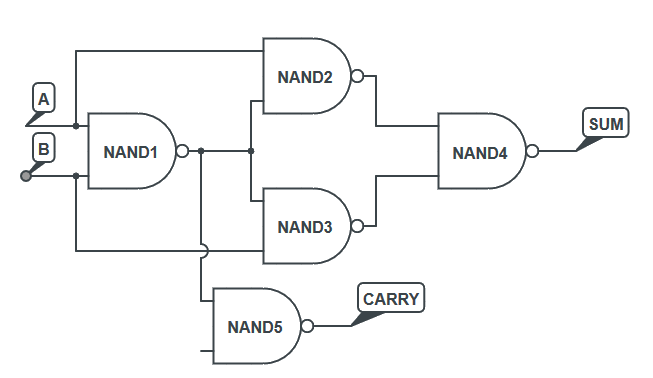
\includegraphics[width=\textwidth]{../grafici/Sommatore1.png}
	\end{minipage}
	\begin{minipage}{0.49\textwidth}
		\centering
		\includegraphics[width=\textwidth]{../grafici/ADDERard.pdf}
	\end{minipage}
	\caption{Schema del sommatore ad un bit e visualizzazione segnali in I/O}
	\label{fig:ADDER}
\end{figure}

\subsection{Osservazione} Negli schemi elettrici mostrati nelle \cref{fig:AND,fig:OR,fig:XOR,fig:ADDER} si può notare che per alcune porte NAND si è lasciato un ingresso flottante, quando si voleva usarle come porte NOT. Si è sfruttato infatti il fatto che gli ingressi flottanti delle porte corrispondono ad un valore \code{HIGH}, secondo la logica TTL.
Tenendo conto di questo si ottiene infatti (\code{HIGH-HIGH} $\rightarrow$ \code{LOW}) e (\code{LOW-HIGH} $\rightarrow$ \code{HIGH}), cioè il comportamento richiesto per una porta NOT.

Si sarebbe potuto connettere gli ingressi insieme, così da avere in uscita ancora una volta un NOT, infatti (\code{HIGH-HIGH} $\rightarrow$ \code{LOW}) e (\code{LOW-LOW} $\rightarrow$ \code{HIGH}) secondo la tabella di verità di una porta NAND, ed essere indipendenti dalla logica usata; si è preferito fare così solo per risparmiare qualche connessione sulla basetta e avere un po' più di ordine (fisico, e quindi anche concettuale).

Si è applicato lo stesso metodo anche nei circuito successivi, anche se gli schemi dei circuiti mostrano gli input connessi insieme perché tratti dalla scheda (vedi \cref{fig:MONO,fig:AST,fig:SQGEN}).

\section{Multivibratore MONOSTABILE}

\begin{figure}[H]
	\centering
	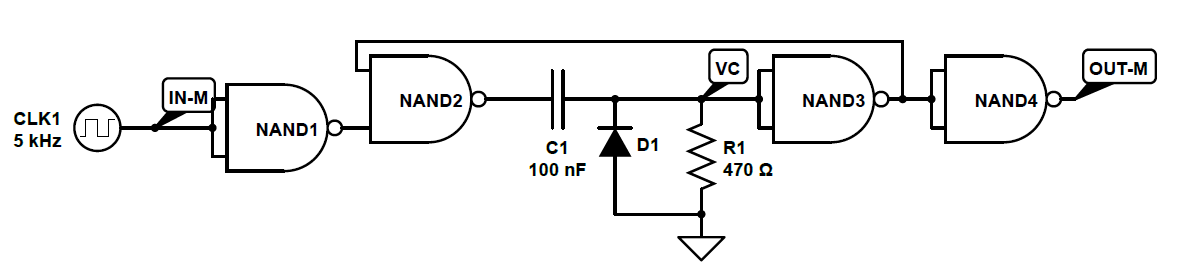
\includegraphics[width=0.9\textwidth]{../grafici/Monostabile.png}
	\caption{Schema del circuito del multivibratore monostabile}
	\label{fig:MONO}
\end{figure}

\section{Multivibratore ASTABILE}

Si è montato il circuito in \cref{fig:AST}.

\begin{figure}[H]
	\centering
	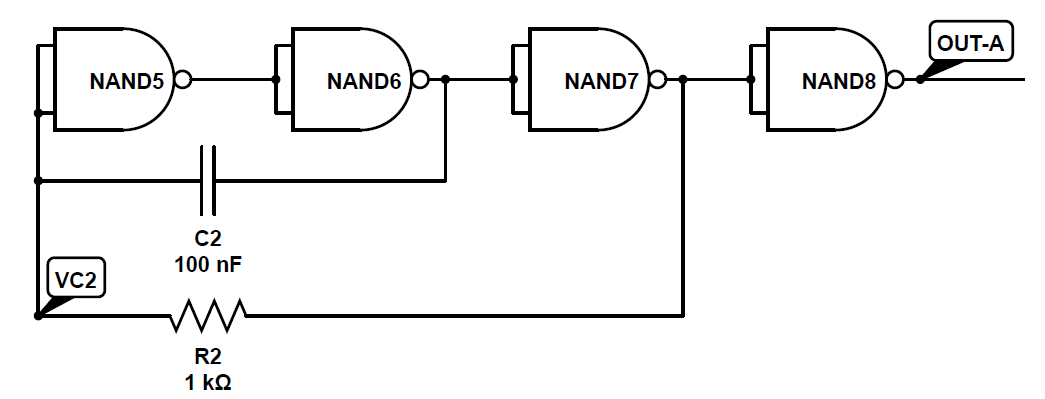
\includegraphics[width=0.7\textwidth]{../grafici/Astabile.png}
	\caption{Schema del circuito del multivibratore astabile}
	\label{fig:AST}
\end{figure}

I componenti impiegati sono stati misurati con il tester, e sono:

\begin{table}[H]
	\centering
	\begin{tabular}{cc}
		$R_2 = \unit{990 \pm 10}{\ohm}$ & $C_2 = \unit{109 \pm 5}{\nano\farad}$\\
	\end{tabular}
\end{table}


\section{Generatore di onda quadra}

\begin{figure}[H]
	\centering
	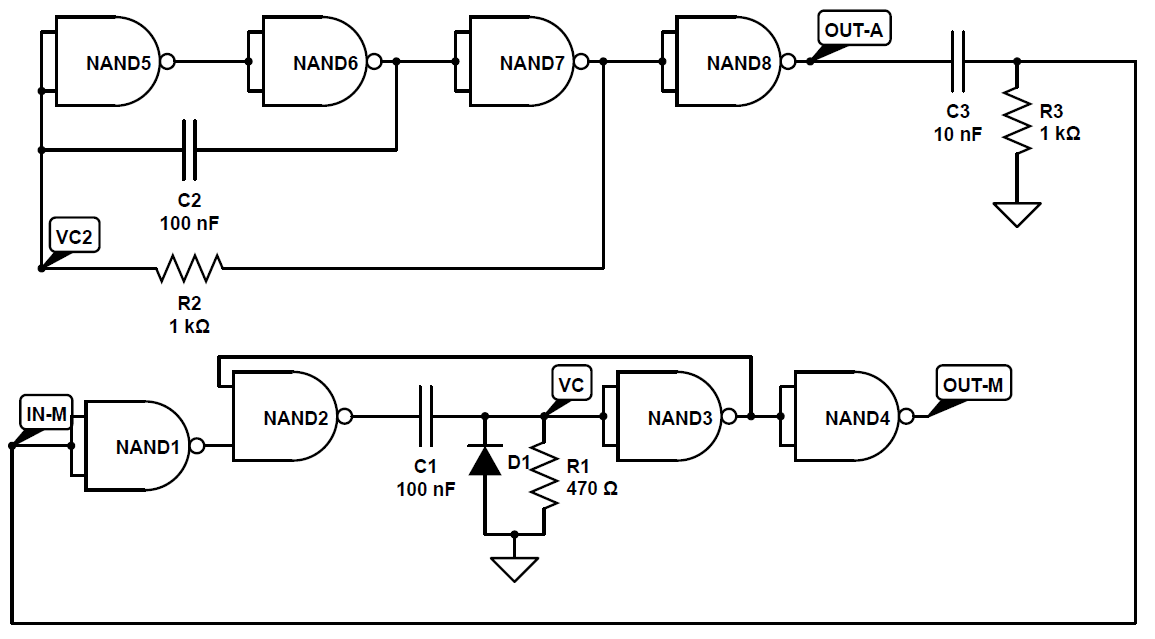
\includegraphics[width=0.8\textwidth]{../grafici/SqGen.png}
	\caption{Schema del circuito del generatore di onda quadra}
	\label{fig:SQGEN}
\end{figure}


\end{document}